\section{Animation}\label{animation}

\subsection{Flight animation - workflow}\label{flight-animation}

In this section there will be explained necessary steps needed to create flight animation. \emph{Flight animation} in Mandelbulber is camera motion track recorded in some kind of flight simulator. The camera can go through interiors of fractal object.
Recording is usually done with low resolution preview. When camera motion track is ready, the animation can be rendered in destination resolution which can be much higher.
Flight animation mode allows to edit every single animation frame in animation table.

\underline{Workflow:}

\begin{enumerate}
	\item Define fractal object (or many objects). 
	
	There has to be selected and configured interesting fractal shape which will present for whole animation. This fractal should have many interesting features and holes where camera could go inside.
	
	The fractal object should be relatively fast for rendering. It is needed because recording of camera flight path will be done in almost real time (or slow motion). 
	
	\item Place camera in start position. Flight will be started from this point.
	
	\item Set low resolution of rendered images. Lower image size will allow to get more frames per second during recording of flight path. There is reasonable to use resolution 320x240 or 160x120
	
	\item disable all effects which can slow down rendering like ambient occlusion, reflections, transparency, volumetric lights, etc. All effects can be re-enabled before final rendering of animation.
	
	\item Open \emph{Flight animation} editor. It can be opened from top pull-down-menu by activating \emph{View} / \emph{Show animation dock}. On the bottom of application window will appear dock with \emph{Flight animation (every frame)} tab (showed below)
	
	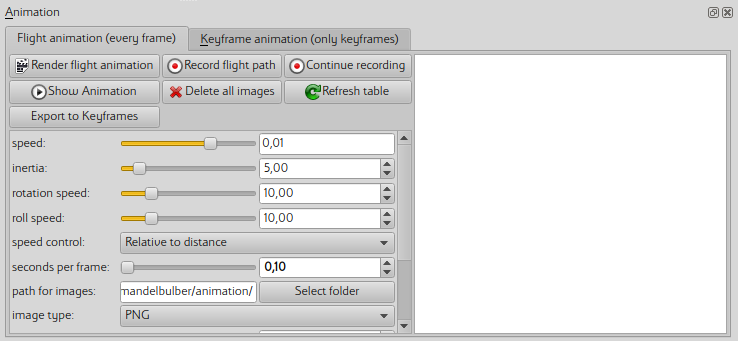
\includegraphics[width=0.7\linewidth]{img/manual/media/flight_animation_dock.png}
	
	\item Set parameters of animation
	
	\begin{description}
		\item[speed] defines how fast the camera will fly. This parameter can be changed during recording of flight path.
		\item[inertia] defines how heavy is the camera. Heaviest camera will make smoother motion, but will be more difficult to control.
		\item[rotation speed] defines speed of reaction for mouse pointer movements. Higher value will allow to turn the camera faster.
		\item[roll speed] defines speed of reaction for Z and X keys which rotate the camera
		\item[speed control] defines how the speed of the camera will be controlled.
		\begin{itemize} 
			\item In \emph{Relative to distance} mode, camera speed will decrease when camera is nearer to the fractal surface. This mode will help you to not collide with the fractal. In this mode you can still control speed by speed parameter and by mouse buttons.
			\item In \emph{Constant mode}, the camera speed is only controlled by speed parameter and mouse buttons
		\end{itemize}
		\item[second per frame] defines frame rate during flight path recording. Higher values give slower rendering but images are more detailed. Value of this parameter is used only during recording and is ignored during rendering of final animation.
		\item[path for images] defines where rendered animation frames will be stored.
		\item[image type] defines image format for rendered frames. Detailed settings for image format are in \emph{File} / \emph{Program preferences}
		\item[show thumbnails] enables previews of frames in animation table
		\item[add flight and rotation speed to parameters] enables possibility to continue recording of animation after recording is completely stopped. 
	\end{description}

	\item Press \emph{Record flight path} button. After 3 seconds recording will be started. During this 3 seconds waiting time the mouse cursor should be placed in the center of image.
	
	\item Use mouse pointer movements to turn camera left / right and up / down. Camera behaves like airplane in flight simulator
	
	Use Z and X key to rotate the camera
	
	Use arrow keys to move camera left / right / up / down. Without \emph{Shift} key camera still goes forward (movement at 45 degree angle). With \emph{Shift} key the camera is not moving forward (movement at straight angle)
	
	Use left mouse button to increase flight speed or right button to decrease speed.
	
	\item Press \emph{space} key to pause recording. When recording is paused, animation parameters can be changed. 
	
	\item Press \emph{STOP} button to stop recording. It's good to pause recording (space key) before stopping, because moving mouse pointer towards \emph{STOP} button can turn the camera.
	
	\item Recording of animation can be continued if \emph{add flight and rotation speed to parameters} is enabled. If \emph{Continue recording} is pressed, recording of flight will start from the point stored in last frame. Camera linear and rotation speed will be maintained.
	
	\item Increase image resolution and enable all needed effects. There can be added light sources, fog, materials, textures, etc.
	
	\item Press \emph{Render flight animation} to do final rendering of animation. It can take very long time depending on image resolution and number of frames.
	
	Rendering of animation can be stopped at any time and continued later. When \emph{Render flight animation} is pressed, there will be rendered only these frames which are missing in folder with animation image frames. Already rendered frames will be skipped.
	
	\underline{Possible additional operations}
	
	%TODO adding of parameters to animation, manual editing, deleting of frames
	
\end{enumerate}

\subsection{Keyframe animation - workflow}\label{keyframe-animation}
